\documentclass{article}
\usepackage[a4paper, margin=1in]{geometry}
\usepackage{graphicx}
\usepackage{caption}
\usepackage{subcaption}
\usepackage{csquotes}

\begin{document}

\title{Image Presentation for the MiniGames Arduino Project}
\author{Fabian Stiewe}
\date{\today}
\maketitle

\newpage

\section{Introduction}
This document is to present the images from the project in real life. I tried to build a minimal box, which included all necessary Arduino components. Even though the box is quite small, one can play games like \enquote{Simon Says} or \enquote{TicTacToe}.

\newpage

\section{Images}
\begin{figure}[!h]
  \centering
  \vspace*{\fill}
  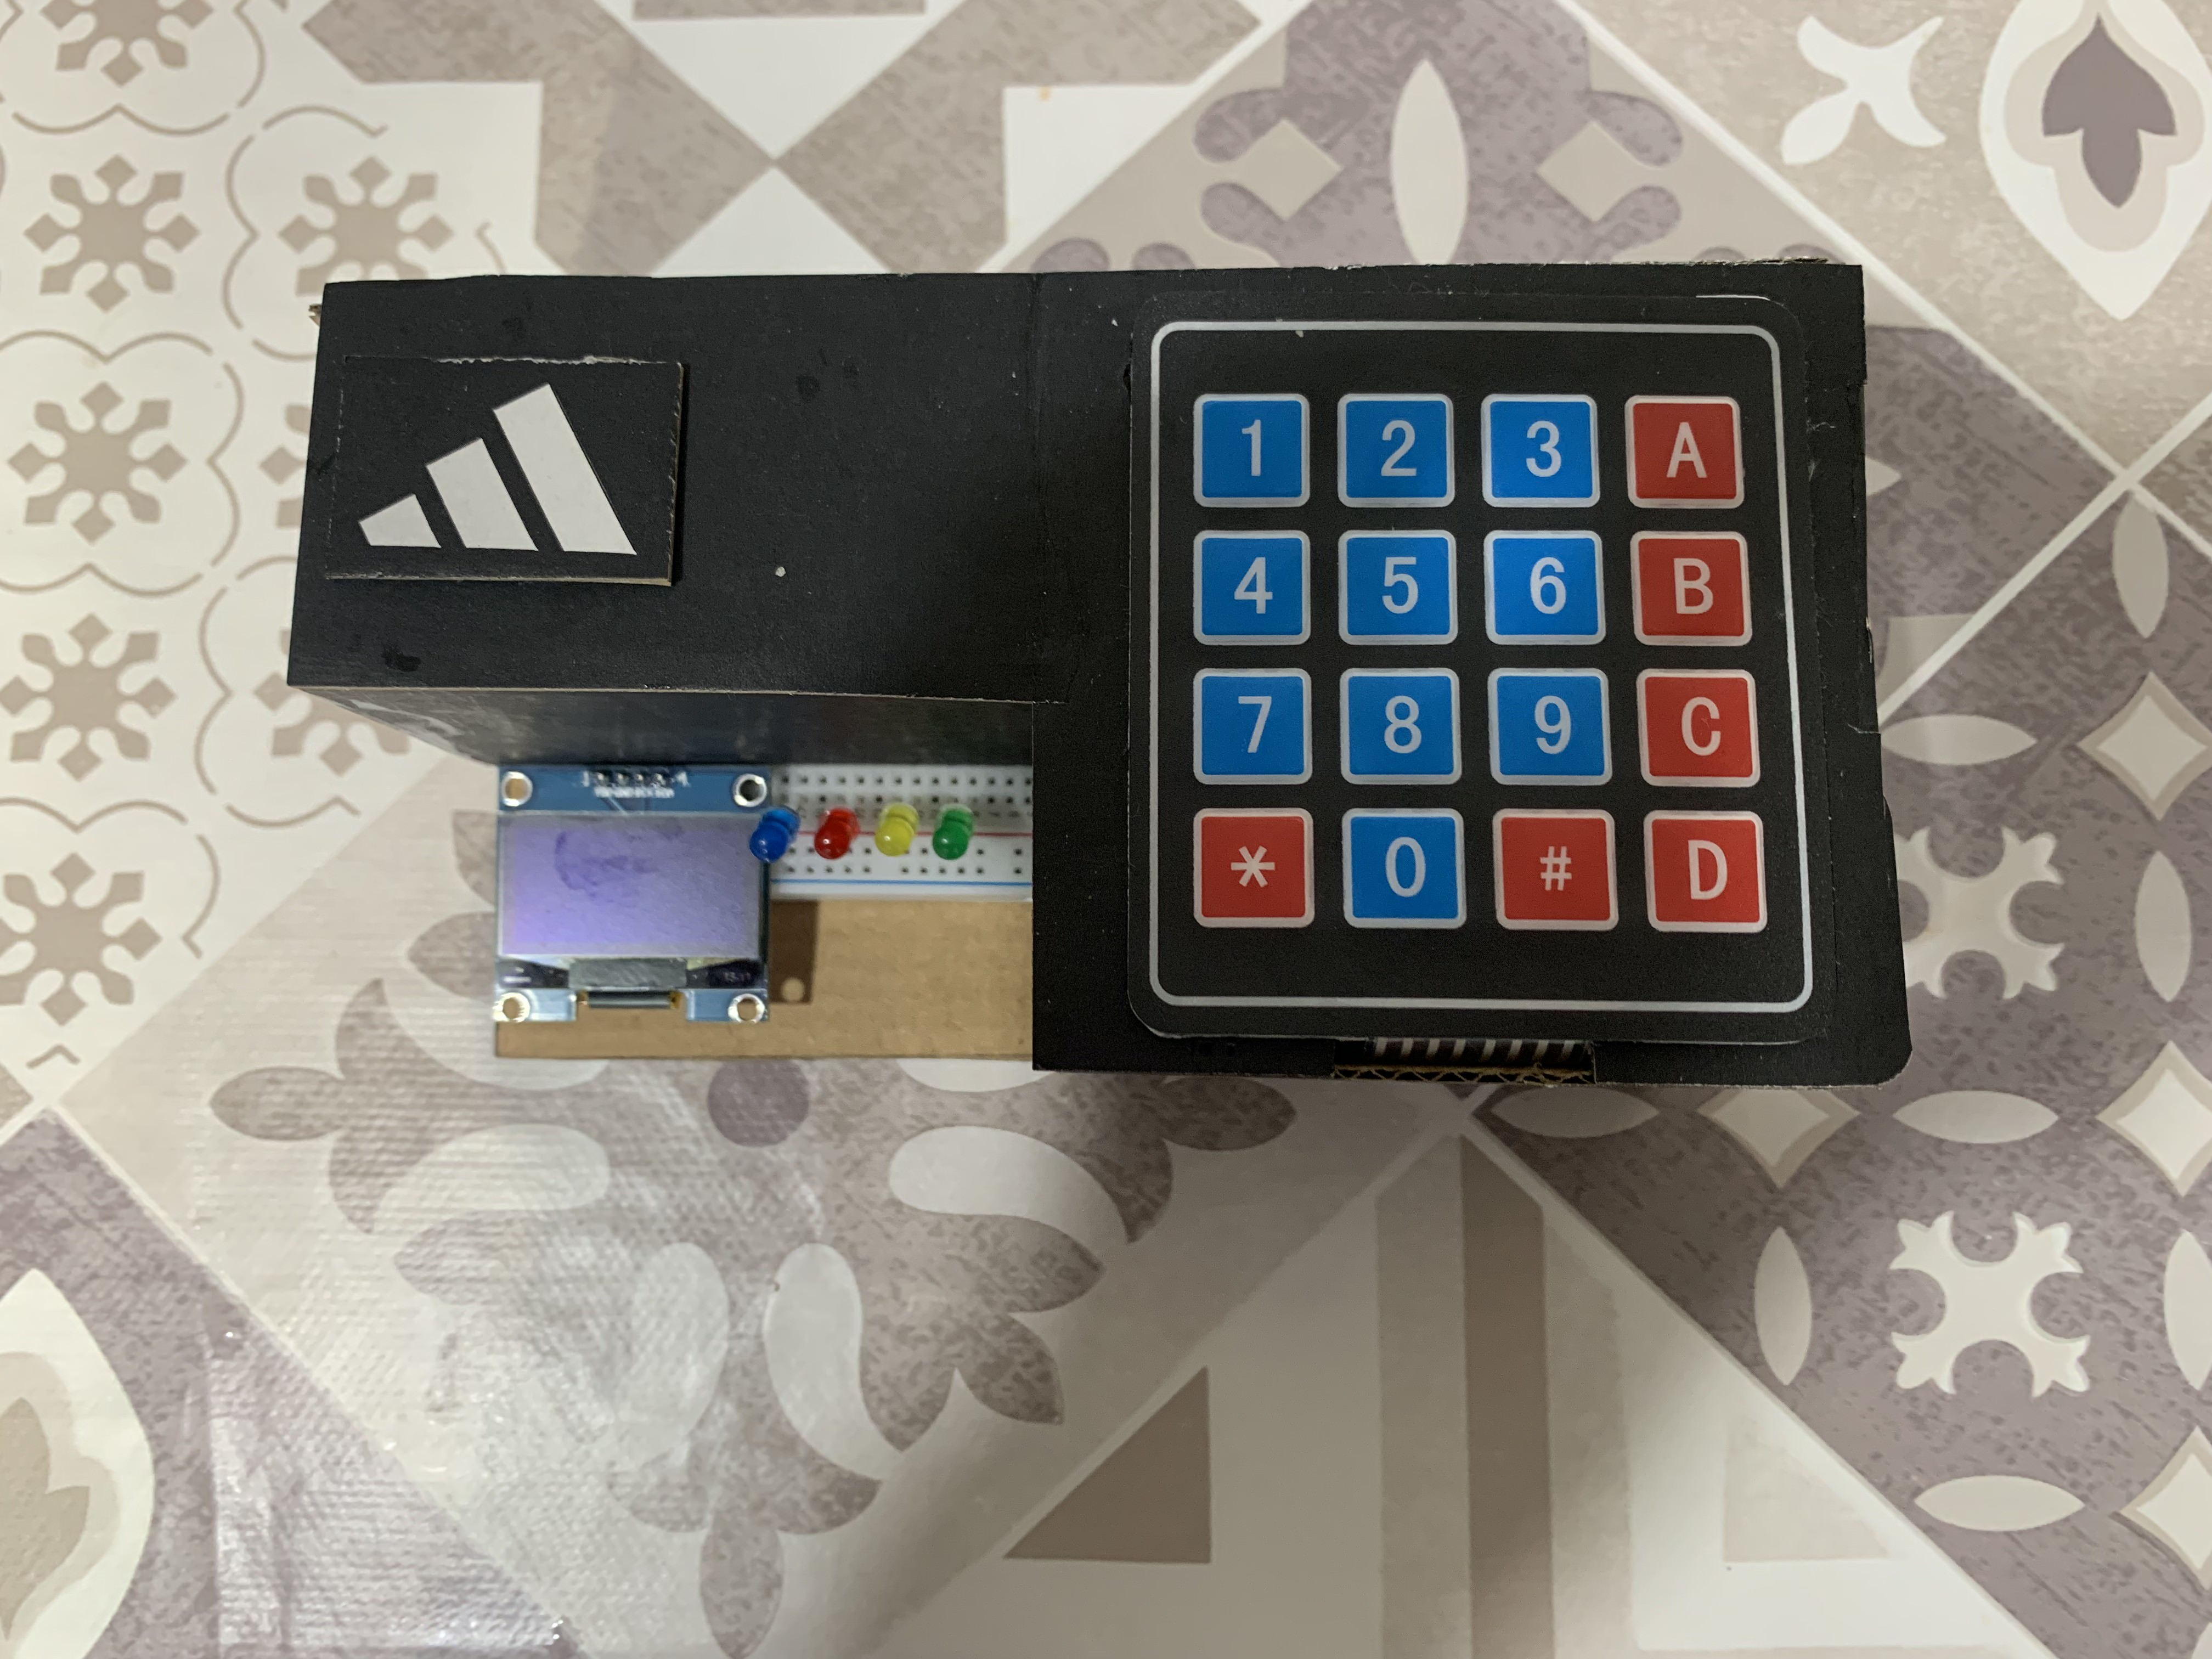
\includegraphics[width=0.9\textwidth]{TopDownView.jpg}
  \caption{Top-down view of the box.}
  \vspace*{\fill}
\end{figure}

\newpage

\begin{figure}[!h]
  \centering
  \vspace*{\fill}
  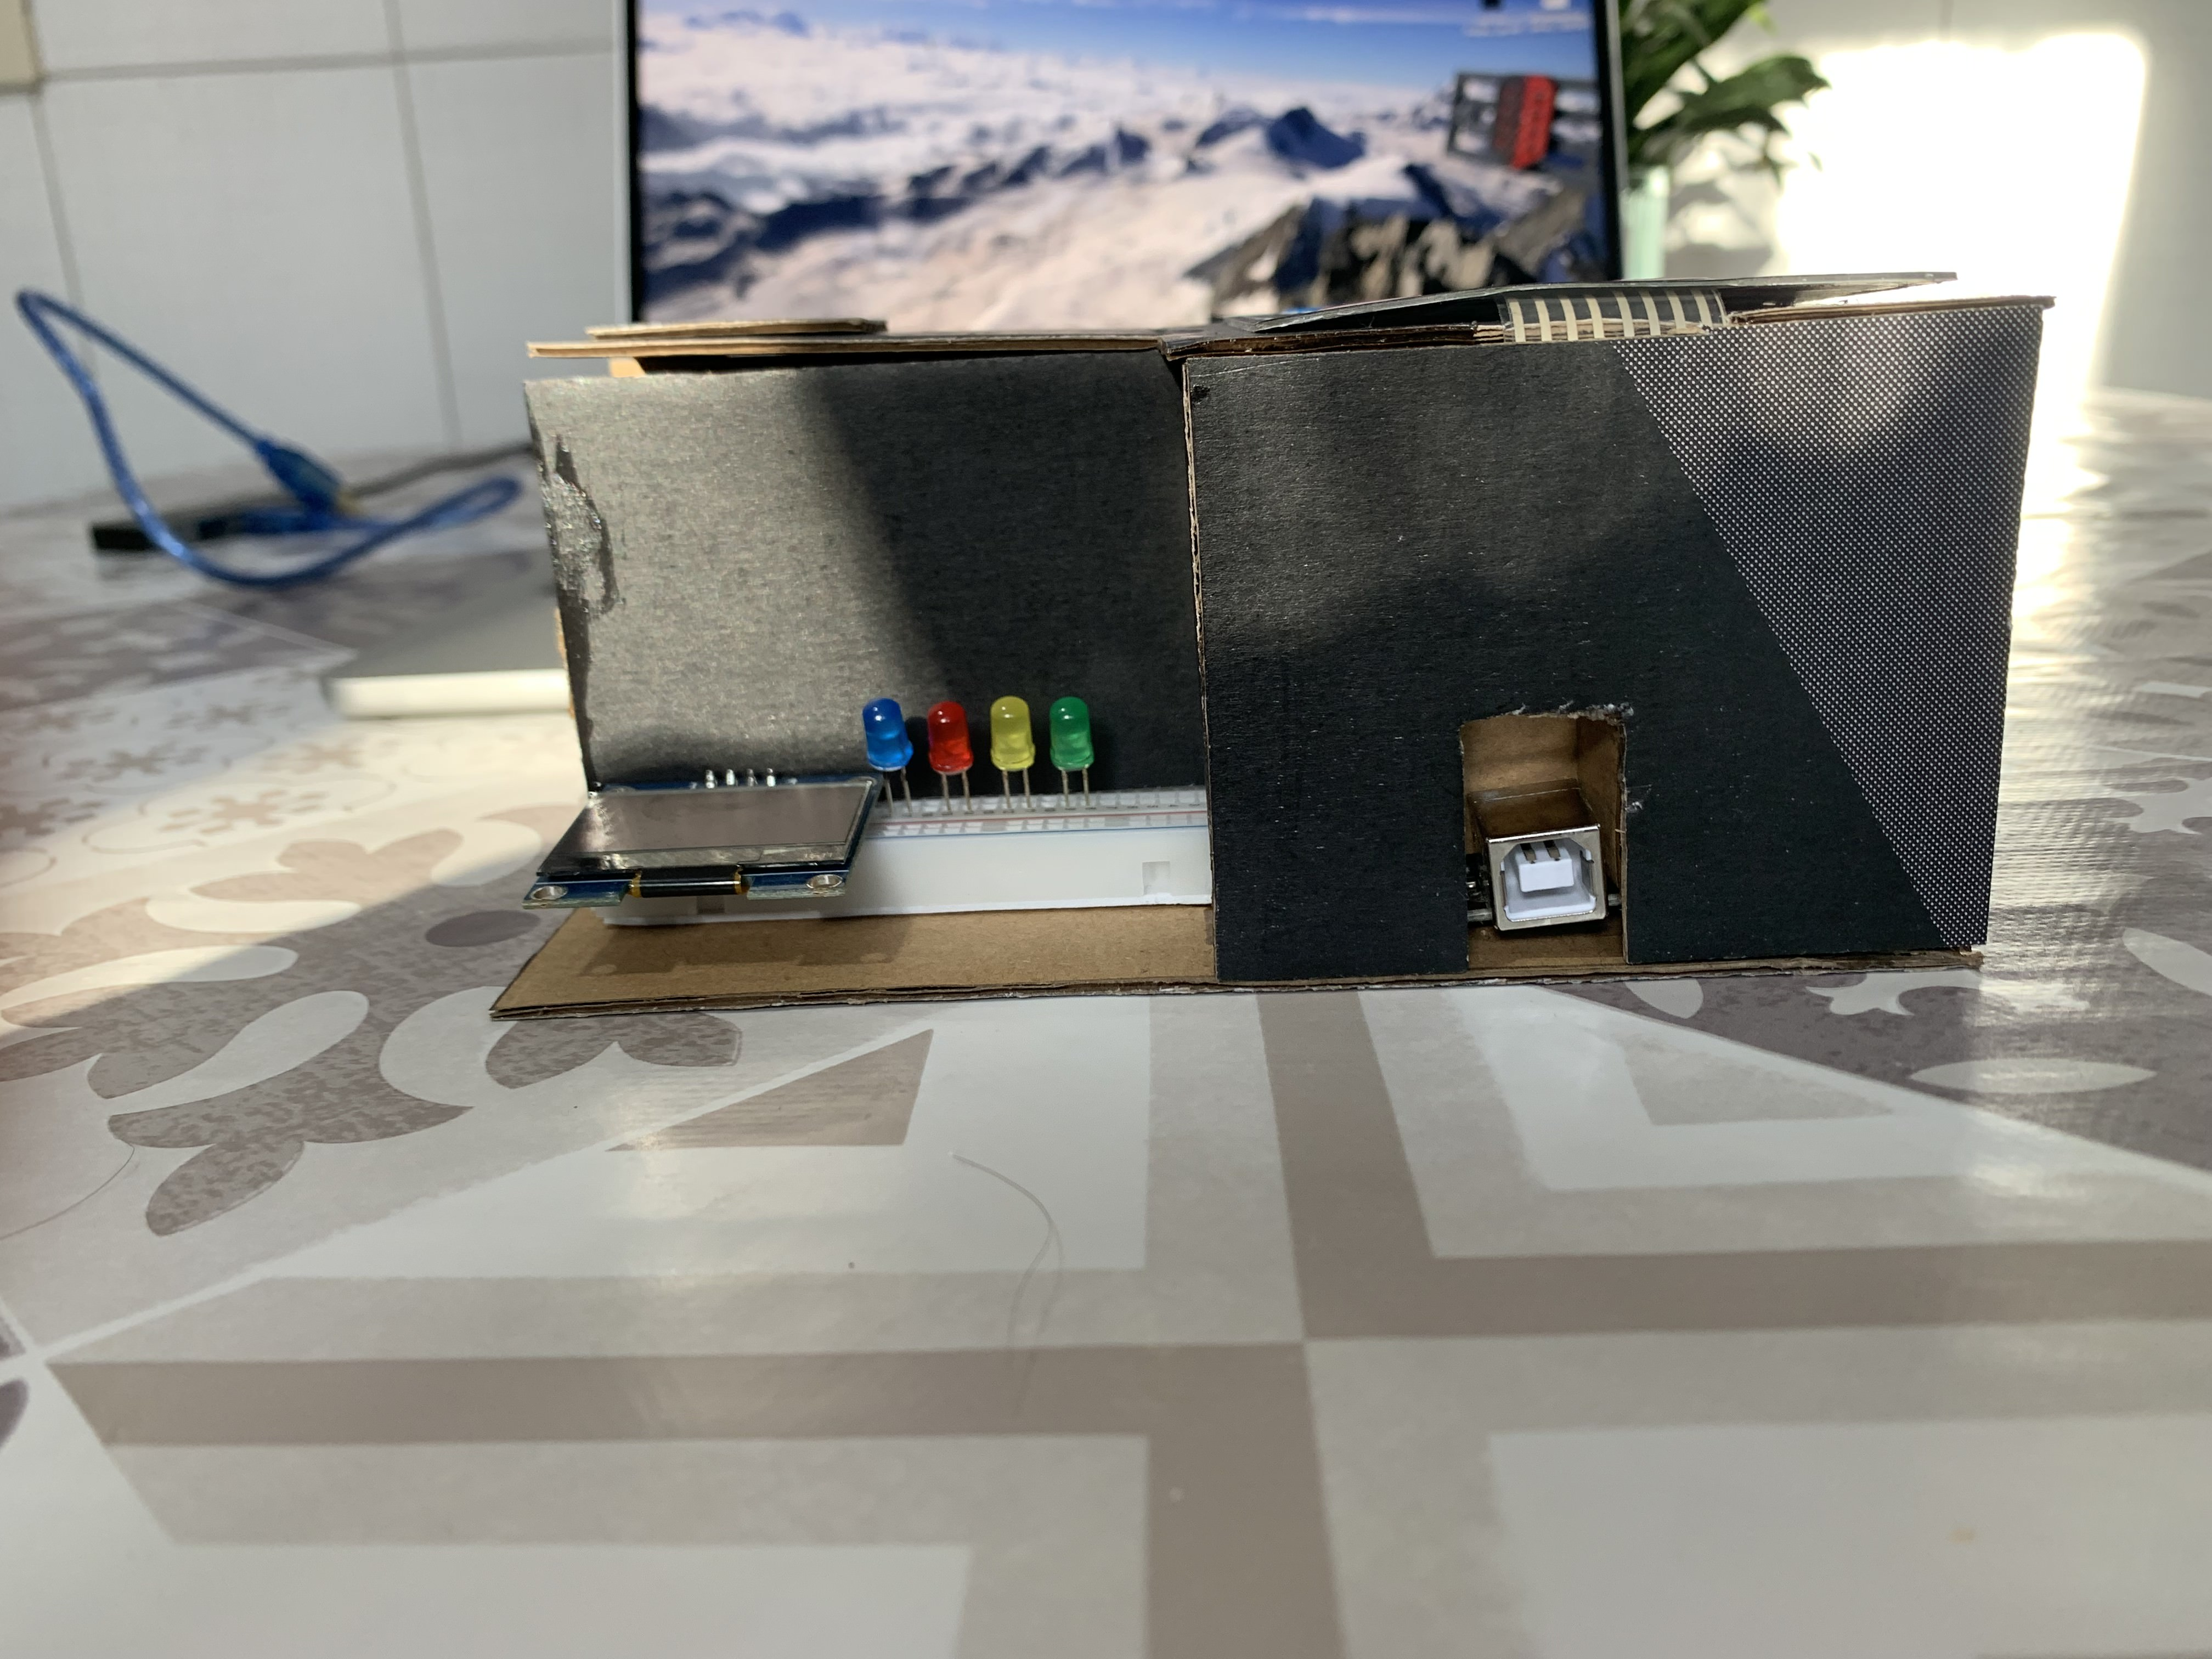
\includegraphics[width=0.9\textwidth]{FrontView.jpg}
  \caption{Front view of the box.}
  \vspace*{\fill}
\end{figure}

\newpage

\begin{figure}[!h]
  \centering
  \vspace*{\fill}
  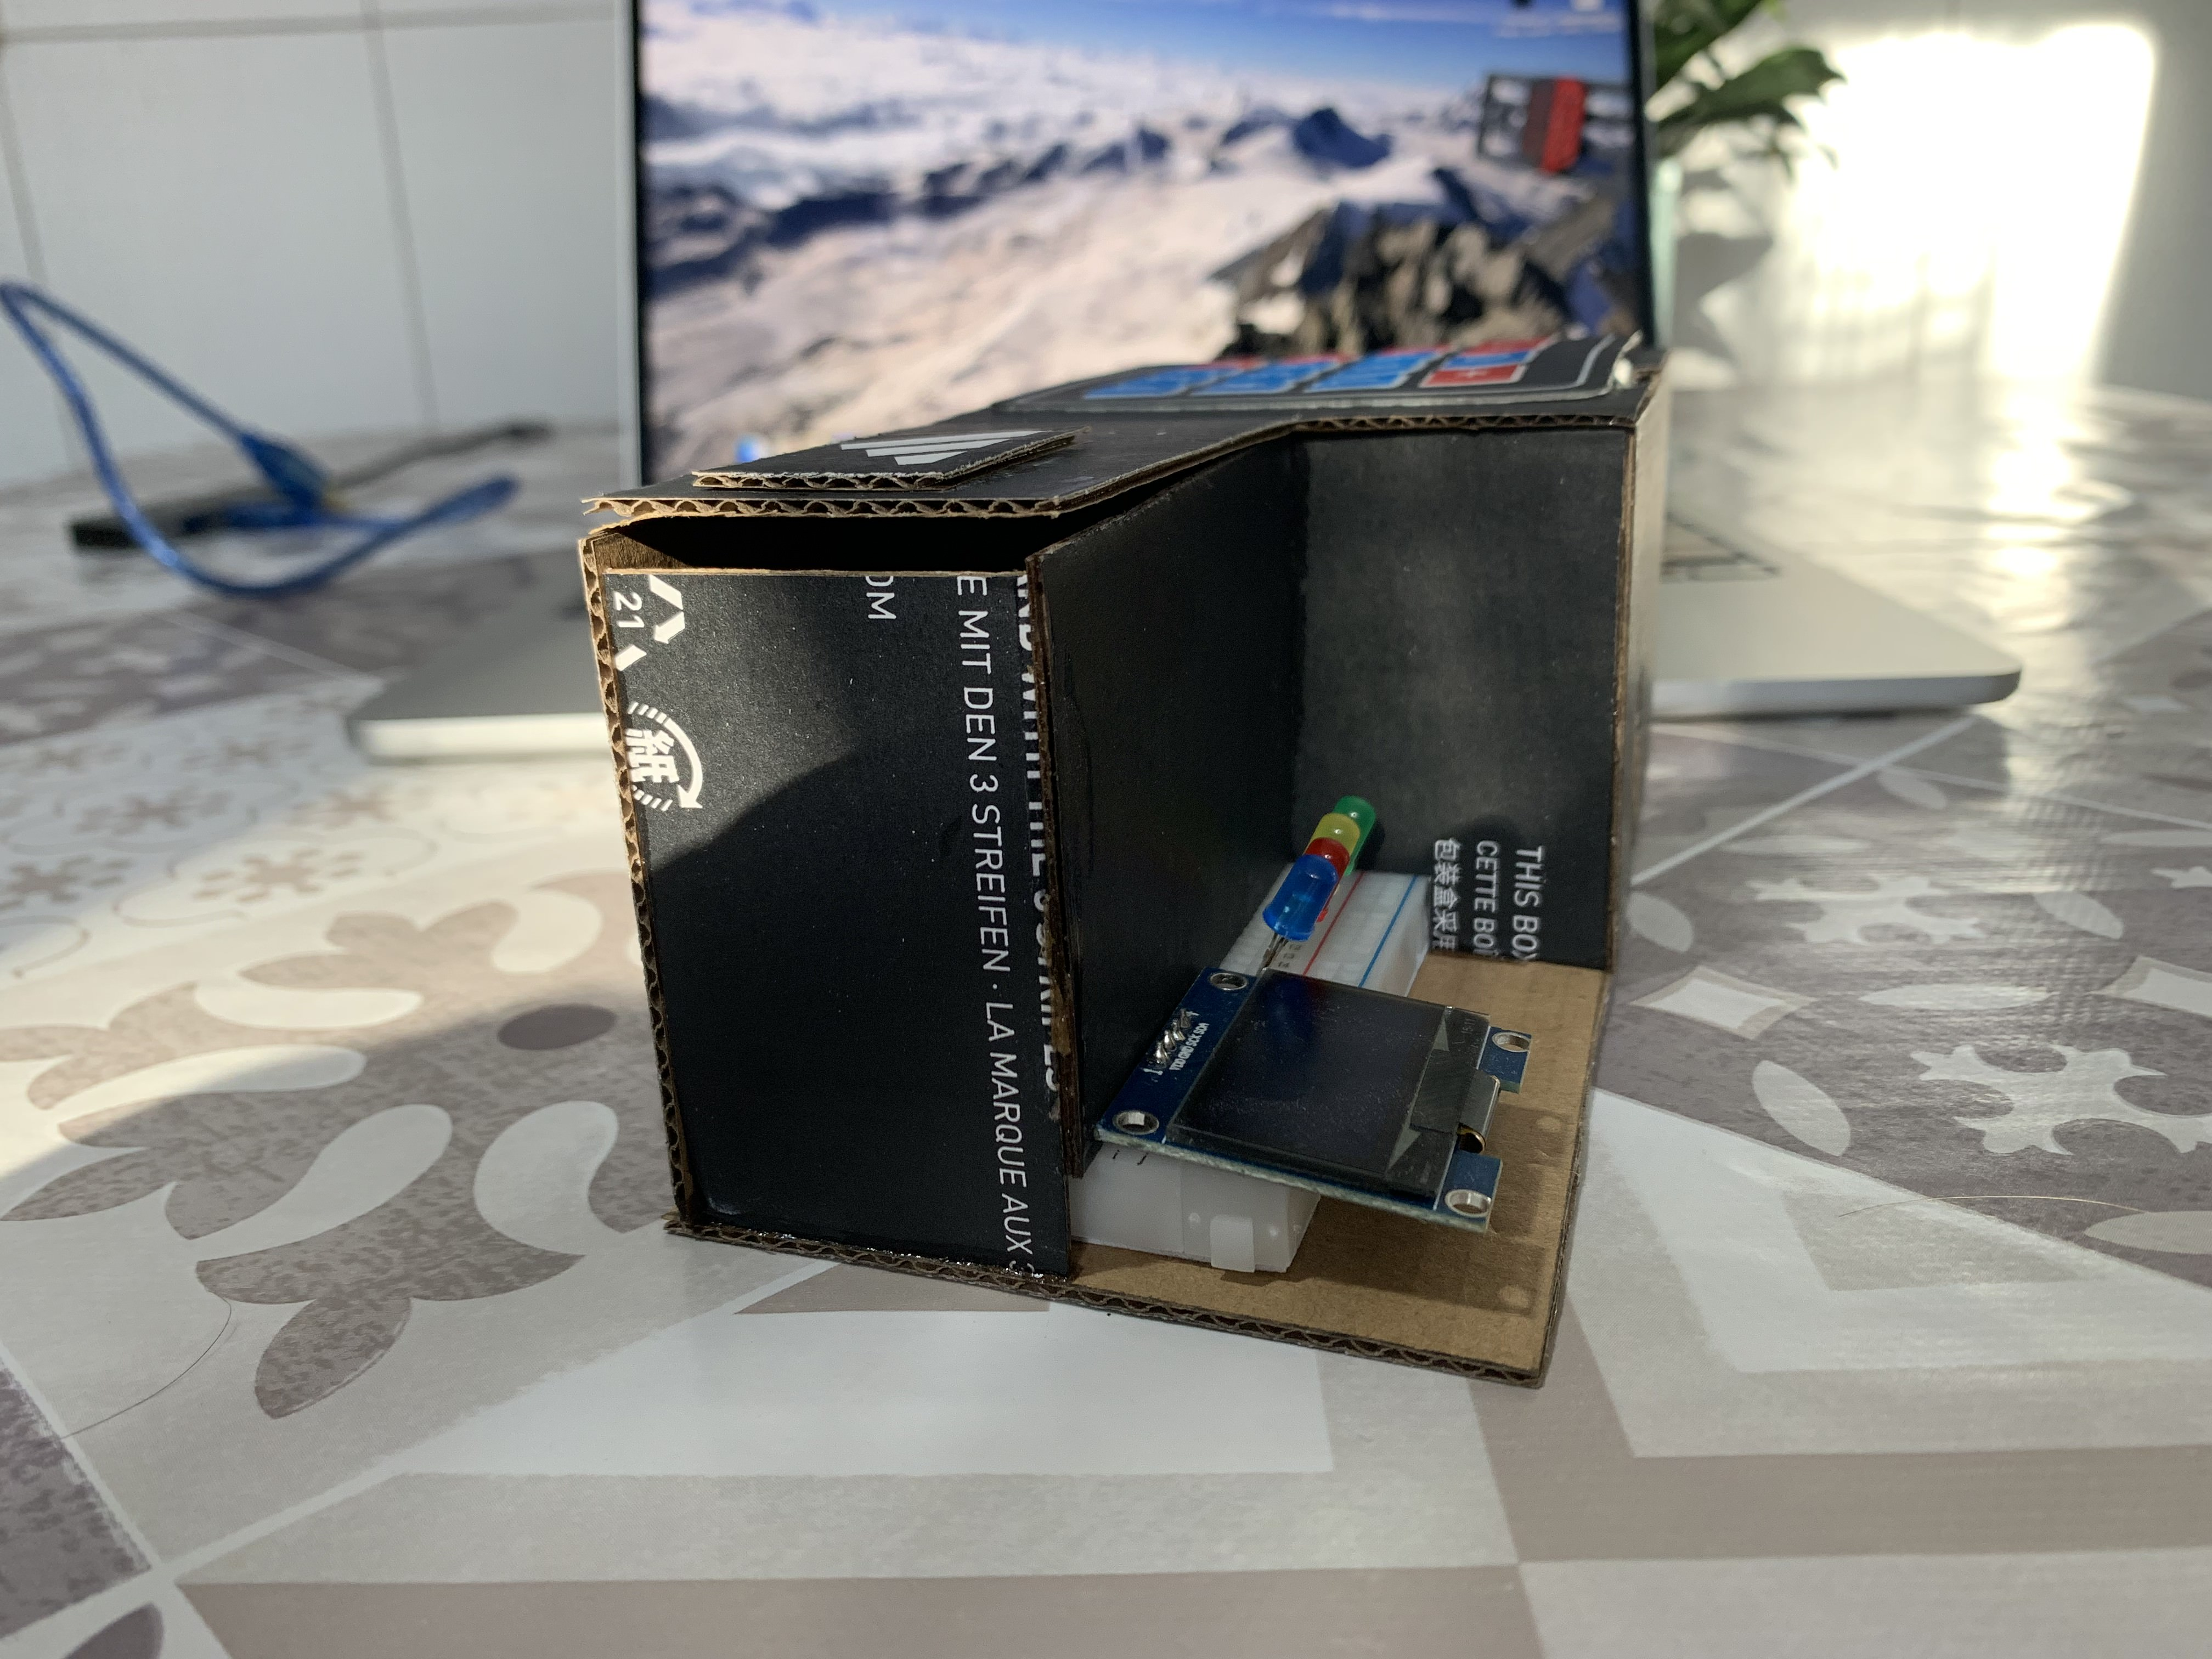
\includegraphics[width=0.9\textwidth]{LeftSideView.jpg}
  \caption{Left side of the box.}
  \vspace*{\fill}
\end{figure}

\newpage

\begin{figure}[!h]
  \centering
  \vspace*{\fill}
  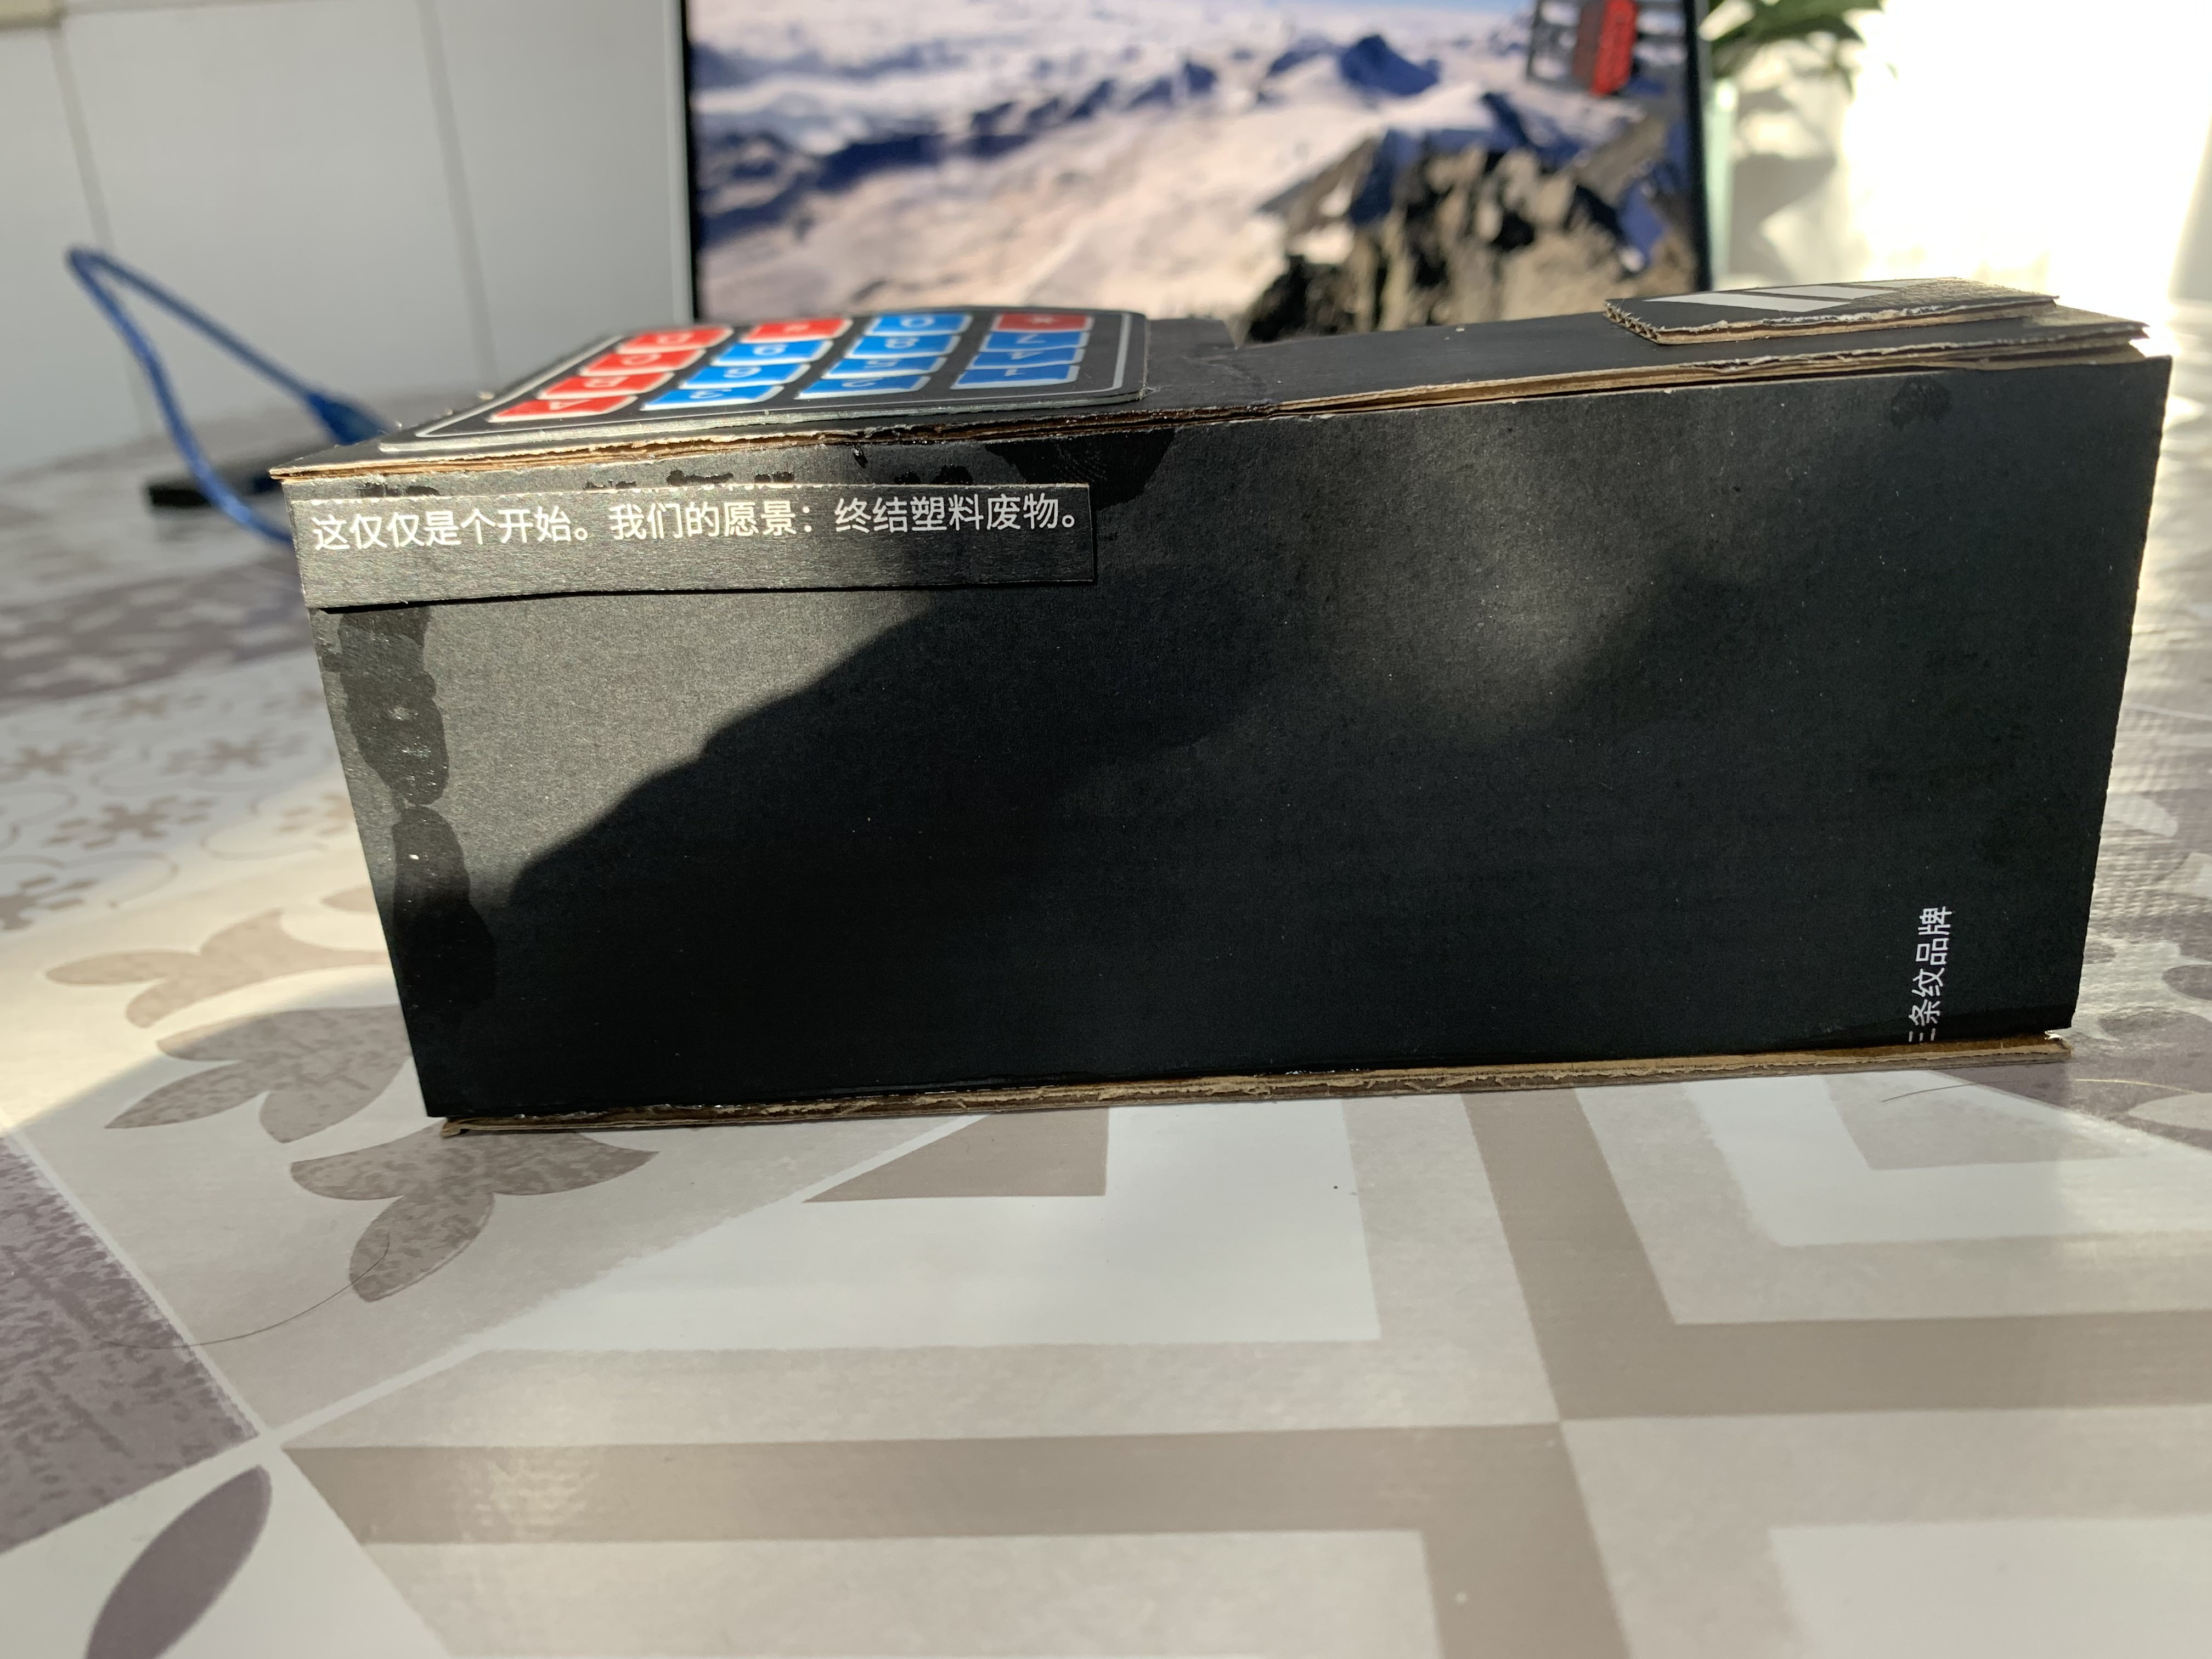
\includegraphics[width=0.9\textwidth]{BackView.jpg}
  \caption{Back of the box.}
  \vspace*{\fill}
\end{figure}

\newpage

\begin{figure}[!h]
  \centering
  \vspace*{\fill}
  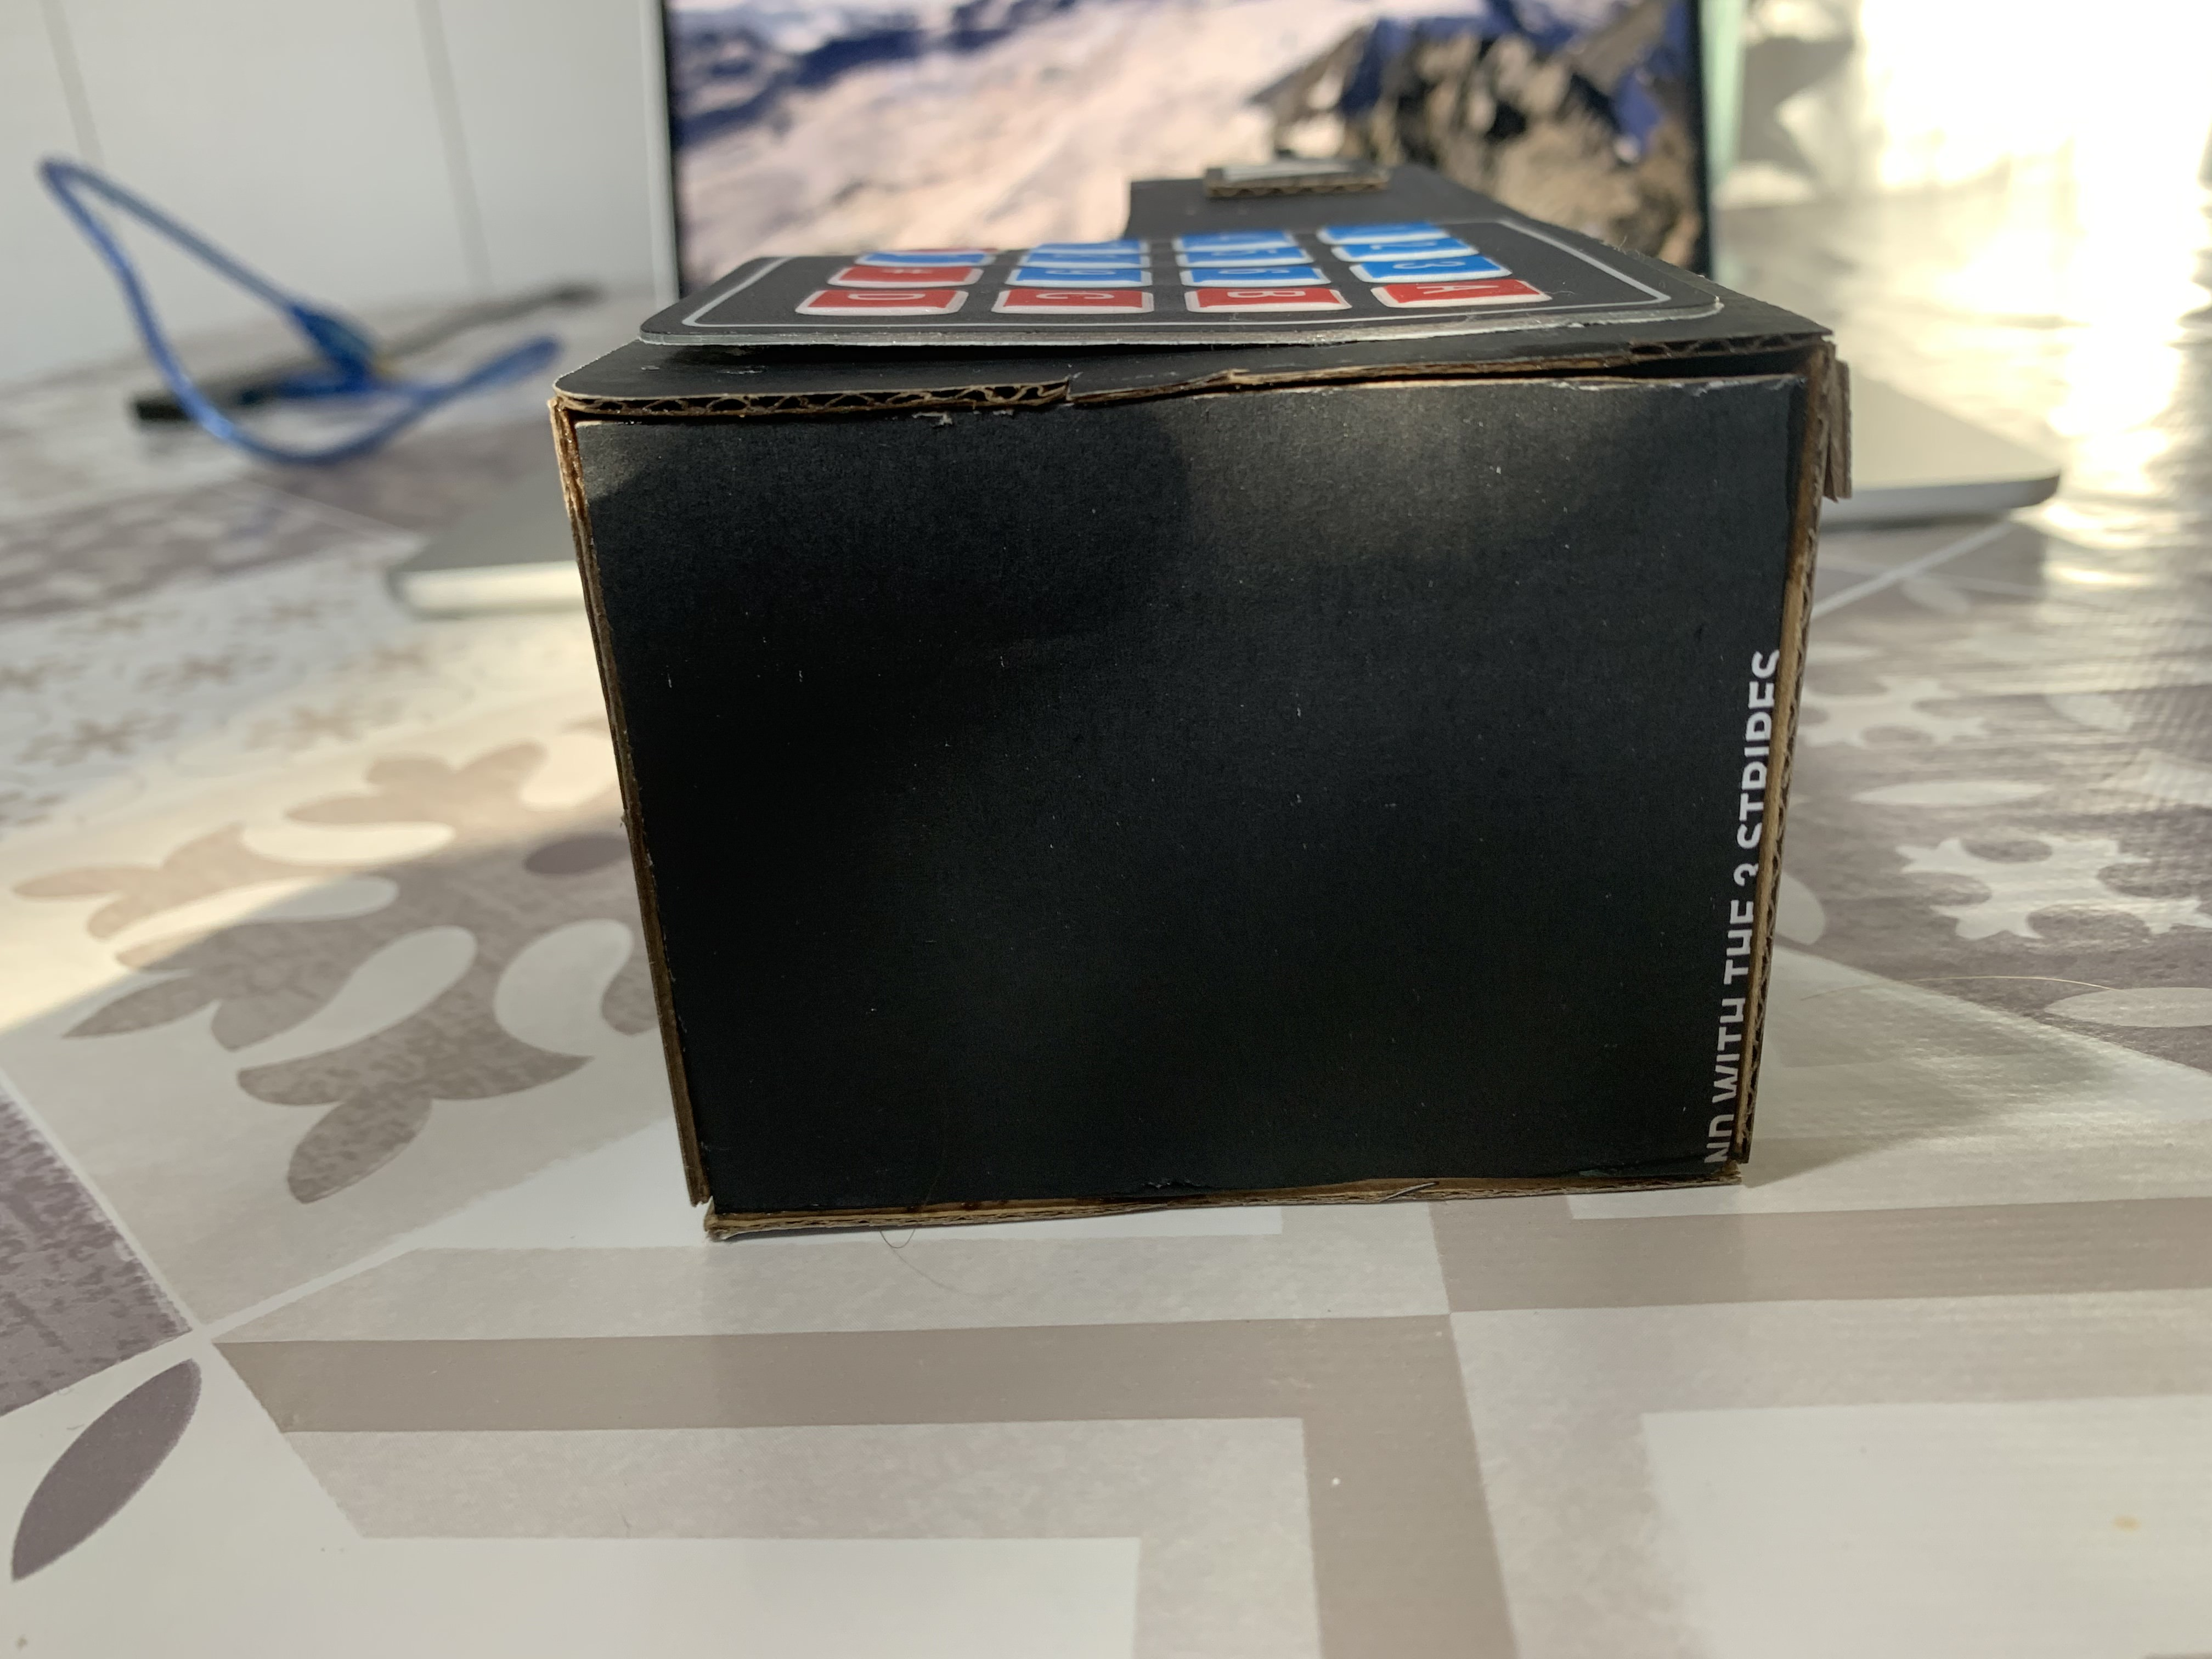
\includegraphics[width=0.9\textwidth]{RightSideView.jpg}
  \caption{Right side of the box.}
  \vspace*{\fill}
\end{figure}

\newpage

\begin{figure}[!h]
  \centering
  \vspace*{\fill}
  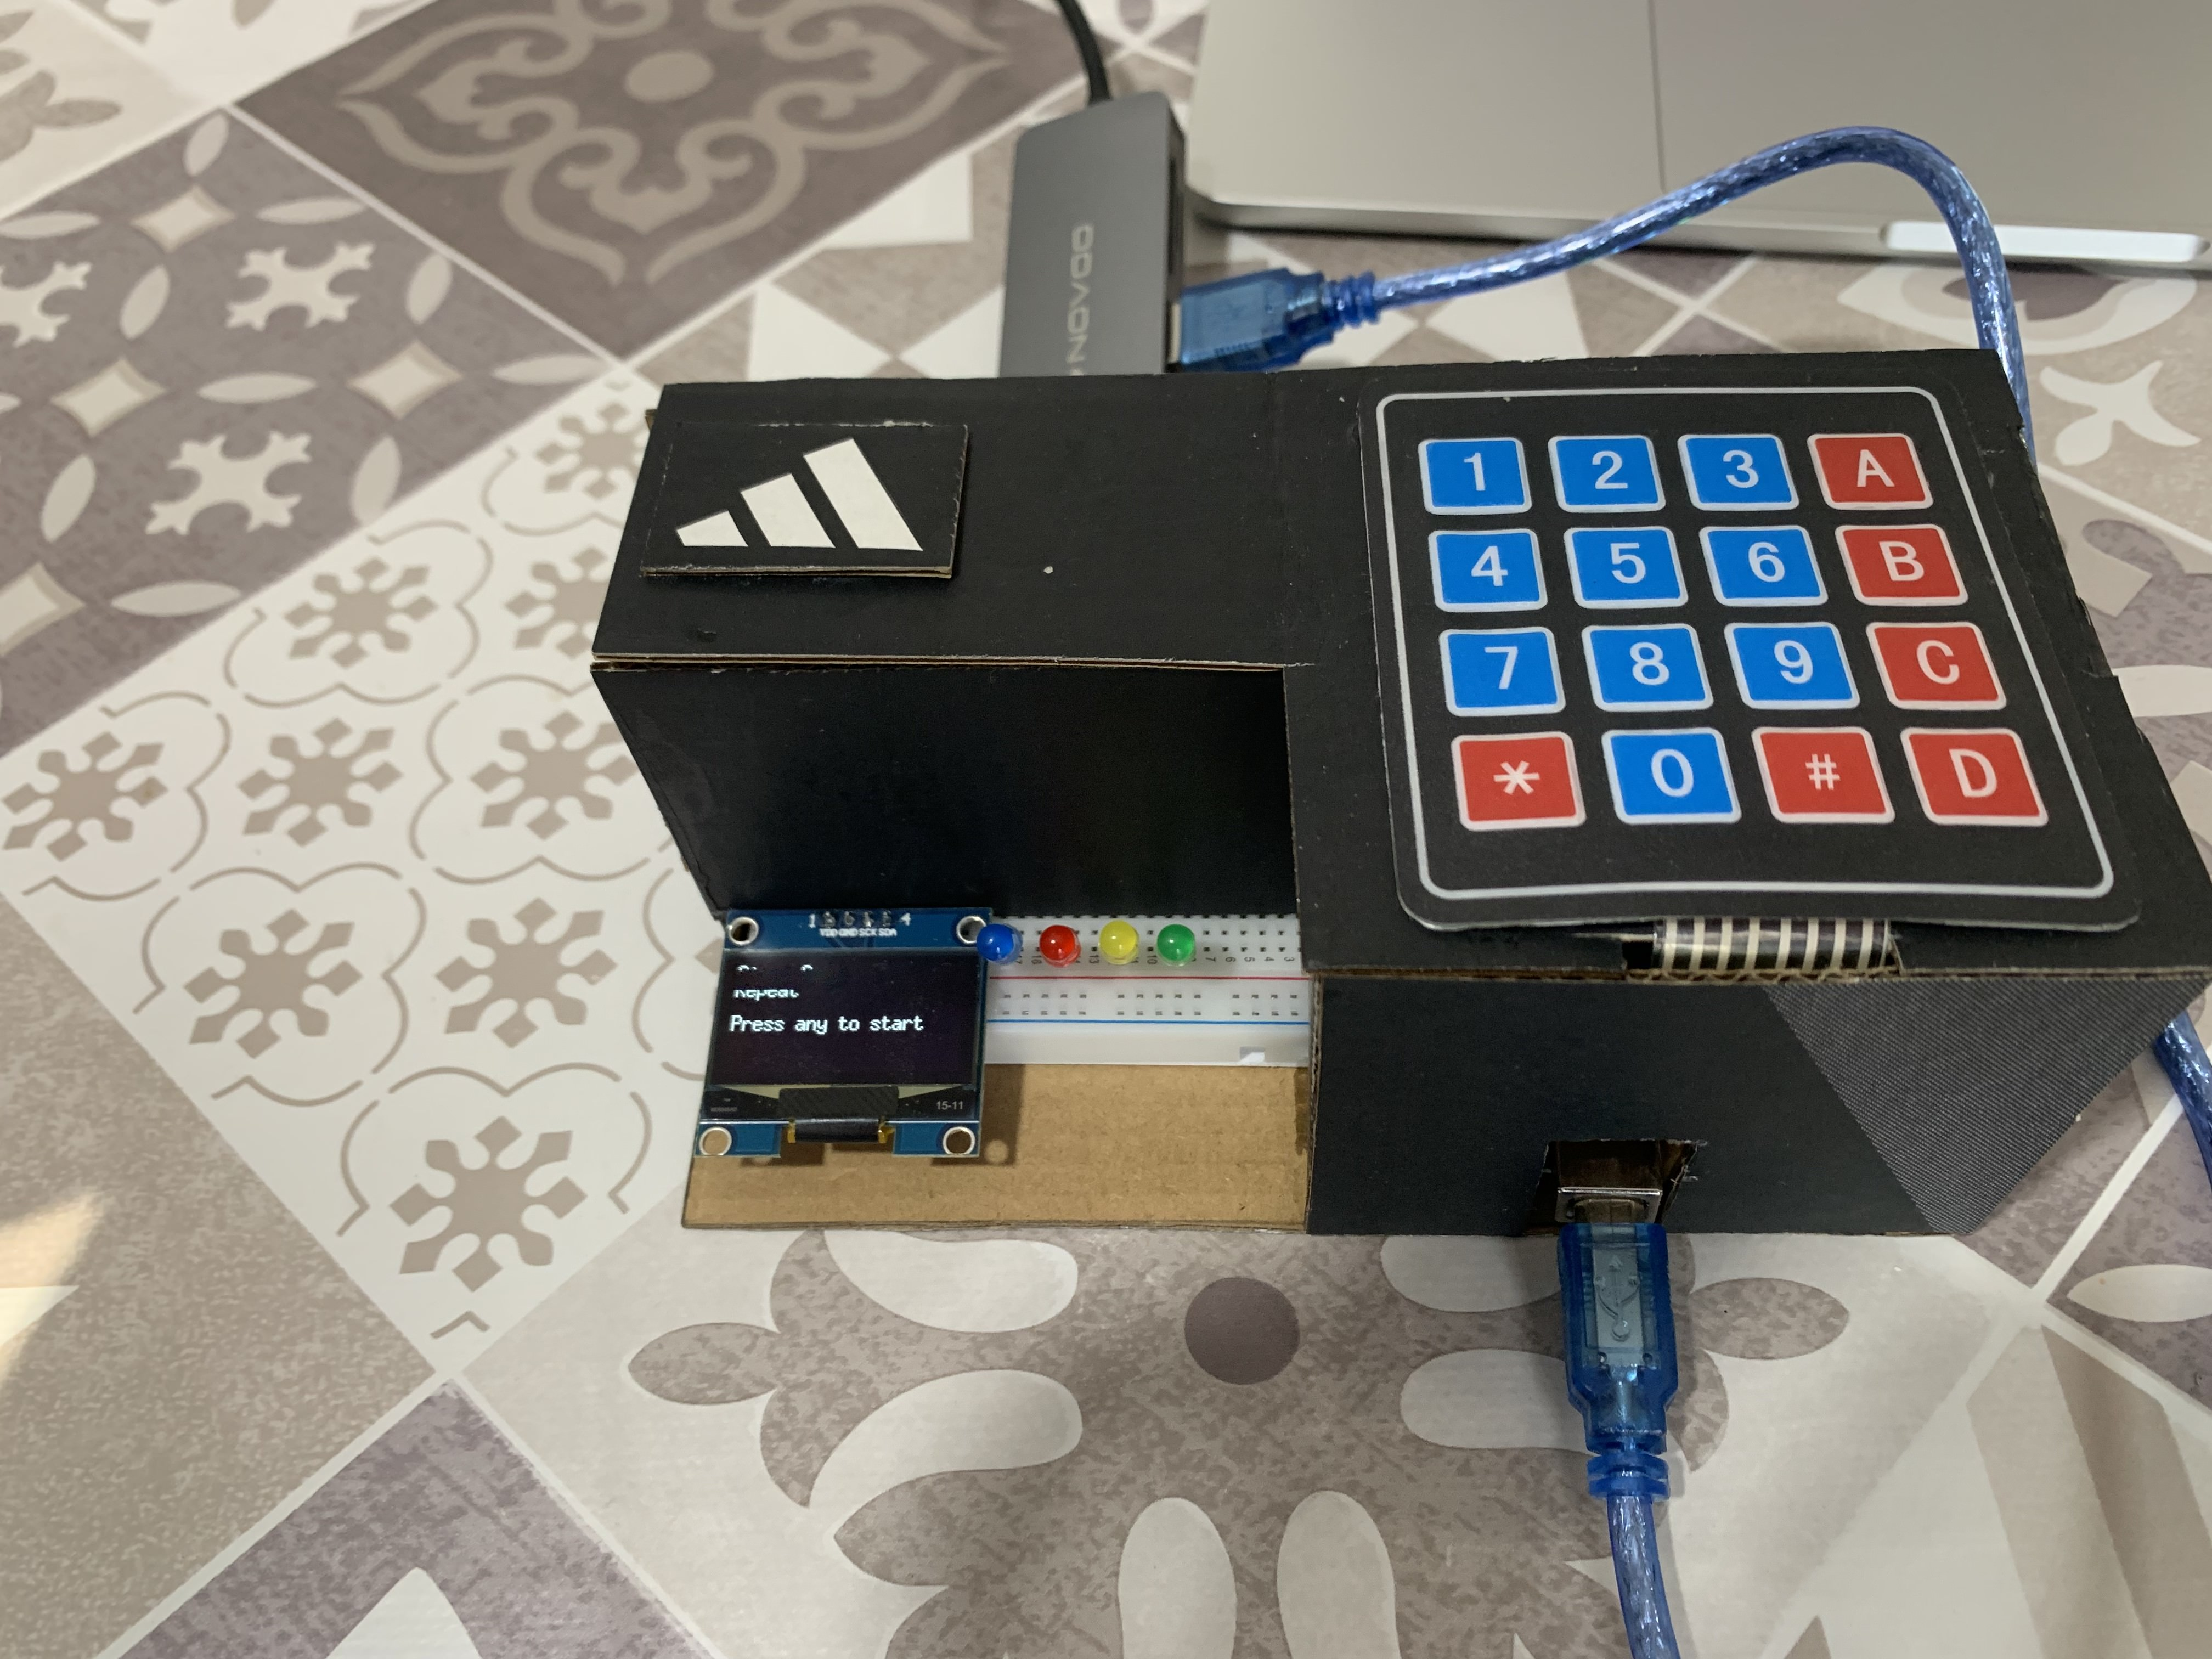
\includegraphics[width=0.9\textwidth]{SimonSaysStart.jpg}
  \caption{Simon Says game start screen.}
  \vspace*{\fill}
\end{figure}

\newpage

\begin{figure}[!h]
  \centering
  \vspace*{\fill}
  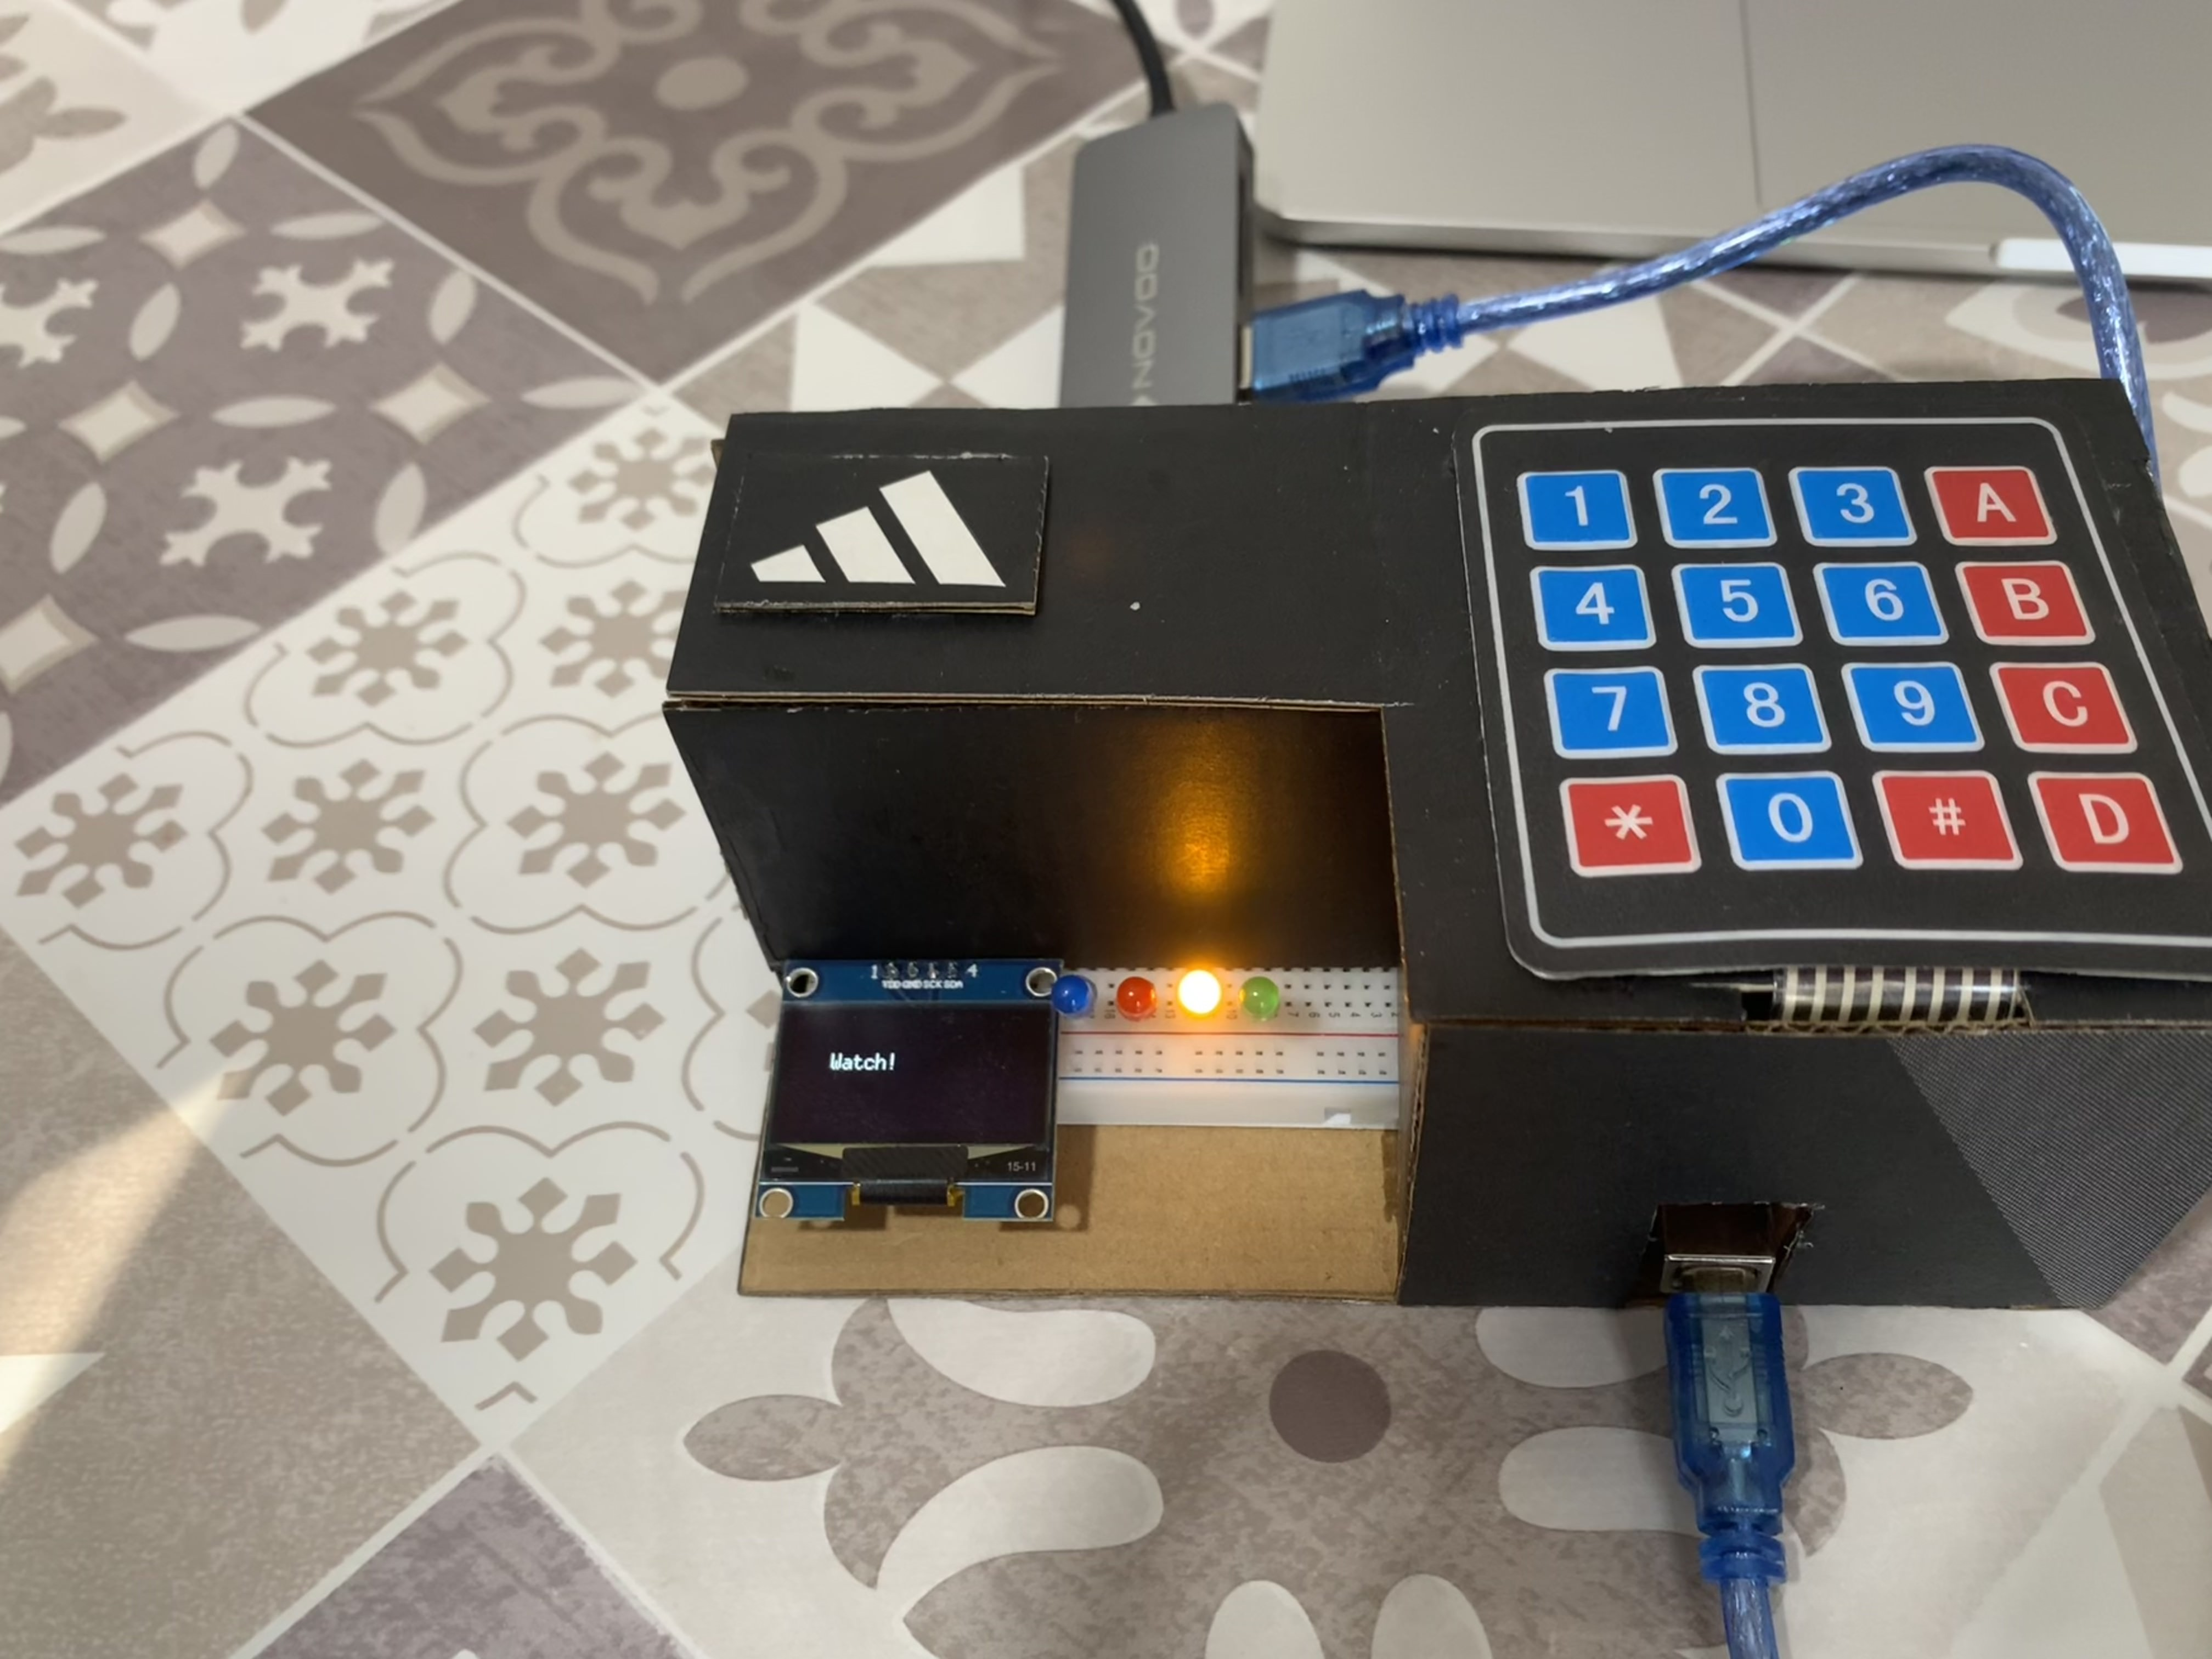
\includegraphics[width=0.9\textwidth]{SimonSaysInGame.jpg}
  \caption{Simon Says game in action. The yellow LED is blinking.}
  \vspace*{\fill}
\end{figure}

\newpage

\begin{figure}[!h]
  \centering
  \vspace*{\fill}
  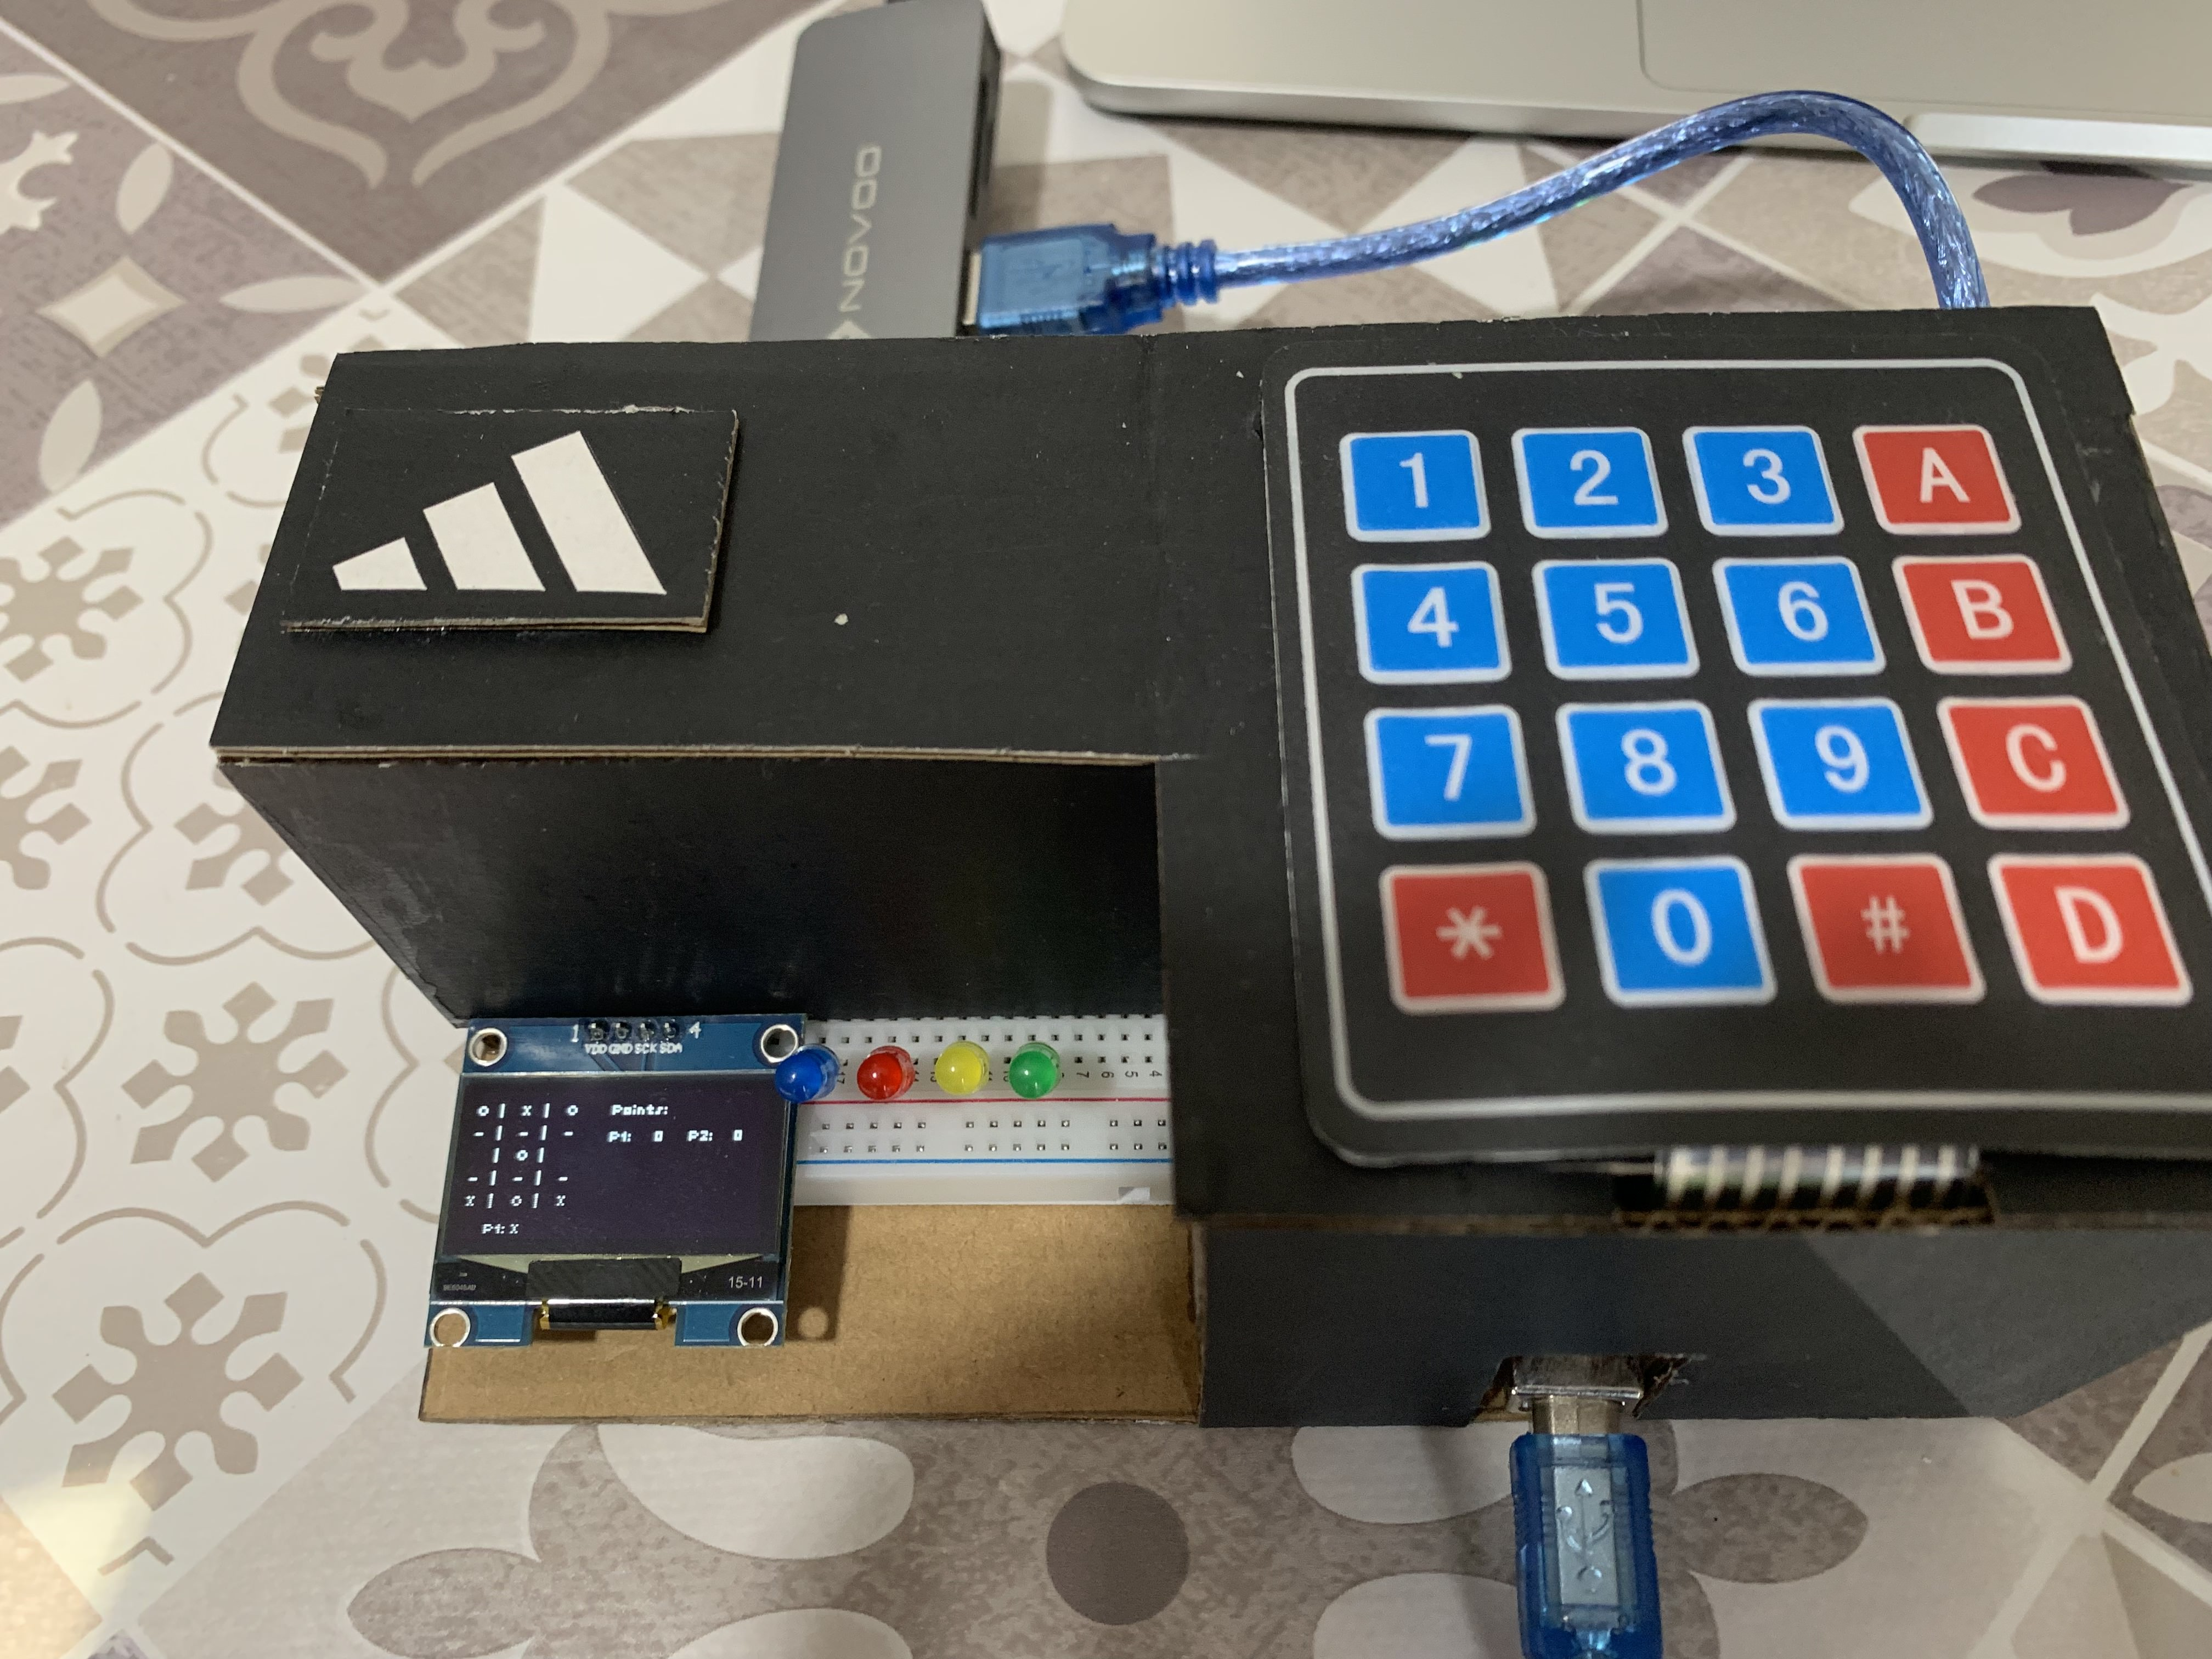
\includegraphics[width=0.9\textwidth]{TicTacToeInGame.jpg}
  \caption{TicTacToe game in action.}
  \vspace*{\fill}
\end{figure}


\end{document}